\section{Graph}
\subsection*{Terminologies}
\begin{enumerate}
    \item vertex, vertice, edge, edges, index, index
    \item Adjacency Matrix, Adjacency List
    \item reachability, connected component
    \item Tree: a connected and acyclic graph, containing backedge and Tree edge.
    \item DAG: Directed Acyclic Graph
    \item Sink(Source): A collection of vertice that doesn't have outgoing(ingoing) edges.
    \item Partition: $C_1,C_2,\ldots ,C_n$ is a partition of $C$ iff their union is C and they don't intersect.
    \item cut: Given a partion {A,B} of P, value defined by $c(A,B)=|E(A,B)|$(number of edges across two sets).
\end{enumerate}

\subsection{Depth First Search}
\subsubsection{Existence of cycles}
Use dfs to traverse all the vertice in a graph. First reach a vertex, then visit its connected component. Most effective when stored in an adjacency list.
Dfs can form a tree(forest).\\
Specially, we analyze the case of directed graph.
For directed graph, there exists 4 kinds of edges: 
\begin{enumerate}
    \item \textbf{Tree Edges} Edges in the DFS search: (u, v) where marked(v) = false
    \item \textbf{Forward Edges} Edges that point to non-child descendants
    \item \textbf{Back Edges} Edges that point to ancestors
    \item \textbf{Cross Edges} All the other edges: edges point to vertices on other tree
    doesn't exist for undirected graph, since if $(c,f)$ occurs it will only be tree edge.
\end{enumerate}

\begin{figure}[htbp]
	\centering
	\begin{minipage}{0.5\linewidth}
		\centering
		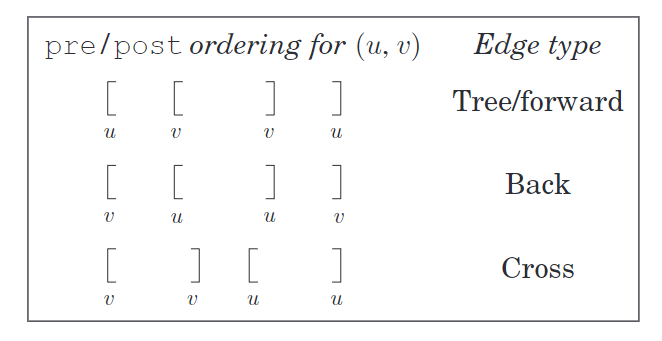
\includegraphics[width=0.8\linewidth]{Notes/fig/edgeType.png}
		\caption{Directed Graph}
        \label{fig:edgeGraph}
    	\end{minipage}
	%\qquad
	\begin{minipage}{0.4\linewidth}
		\centering
		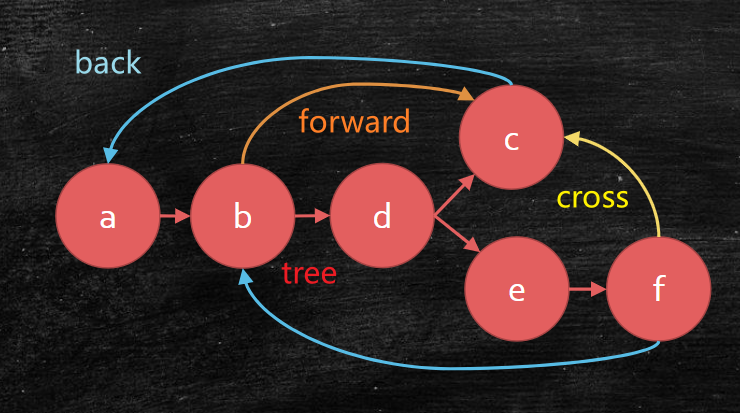
\includegraphics[width=0.8\linewidth]{Notes/fig/edgeTypeFigure.png}
		\caption{colored edges}
		\label{fig:colored}%文中引用该图片代号
	\end{minipage}
\end{figure}
\textbf{Correctness of Algorithm:}

If there exists a back edge in directed graph, a cycle exists.

If a cycle exists, then a backedge must be found. Since a tree is acyclic.

By algorithm \ref{alg:dfs} plus the condition of the existence of a backedge ($pre[v]<pre[u]$ and $post[u]<post[v]$), depicted in \ref{fig:edgeGraph}
\begin{algorithm}
    \caption{DFS on Directed Graph}
    \label{alg:dfs}
    \SetKwFunction{explore}{explore}
    clk=0\\
    \ForEach{$v \in V$}{
        \If{marked[v]=False}{
            \explore{$v$} \\
            clk++ \# used to calculate the number of connected components\\
        }
    }
    \SetKwFunction{explore}{explore}
    \SetKwProg{Fn}{Function}{:}{}
    \Fn{\explore{$u$}}{
        pre[u]=clk\\
        clk++\\
        visited[u]=false\\
        \ForEach{$(u,v) \in E$}{
            \If{marked[v]=false}{
                \explore($v$)
            }
        }
        post[u]=clk\\
        clk++\\
    }
\end{algorithm}



\subsubsection{Application: Topological Ordering}
A DAG must have topological ordering, since:
\begin{enumerate}
    \item Every DAG have a sink.\\
    Intuitively, if we start at $v$, since there exists an outgoing edge for every vertex. Since DAG doesn't have cycles, in finite steps, we'll visit every vertex,
    \item Find a topological order.\\
    When deleting sink vertice and edges pointing to them, we obtain a new DAG. By repeting the operation of finding sink (visiting sink at last), and deleting sink to construct new graph, and finding sink in the new graph... We successfully find a topological ordering by following the inverse sequence of the sinks.\\
\end{enumerate}
\textbf{Time Complexity:}

Finding a sink takes $O(|V|)$, removing a sink to update graph with $|V|$ rounds.

A trick is that the vertice with the earliest post ordering is a sink. If not, the outgoing point points to another vertex that finishes earlier.
(consider the fact that no edge (u,v) exists in DAG that satisfied $post[v] > post[u]$. See \ref{fig:edgeGraph}, backedges satisfy, but doesn't exist in DAG)
Therefore, the topological ordering is the inverse order of finishing points, which brings the time complexity of DFS down to $|E|+|V|$.\\
\textbf{Correctness:}

If (y,x) exists, y is not a sink since x is in the graph, contradiction!


\subsubsection{Strongly Connected Components for Directed Graph}

All the SCC forms a partition of C. i.e. for every $v$, $\exists C_i$ so that $v \in C_i$. For completeness, by construction, every single $v$ can be formed as a SCC. For non-intersection, if $v \in C_i,C_j$, $C_i$ and $C_j$ together forms a bigger C.C., as every vertex from $C_i$ can reach points from $C_j$ through $v$.\\
\begin{itemize}
    \item Note that we can't simply employ DFS to find C.C., as although you find reachable points from a certain vertice $v$, the vertice you explore may not be reachable from each other.
    \item Note that unlike topological ordering, the node with the earliest post time doesn't necessarily occur in sink SCC,
    as the vertice with outer edges are previsited where our algorithm ends in somewhere else.i.e.,for graph \ref{fig:SCC} consider DFS in sequence {5,6,7,8}, apparently, the 8 has the smallest post value, but is not in sink.
    \item However, the vertice with biggest post time must be in source SCC. 
    Assume $u$ has the largest finish time, which must be a root of one DFS tree. Suppose $u$ isn't in source SCC, i.e. $\exists v$ s.t. $(v,u)$ exists. 
    $v$ isn't in the tree of $u$, as $(u,v)$ doesn't exist.
    ,$v$ cannot start earlier than $u$, $v$ isn't in another DFS tree. 
    \item Consider the meta-graph, where connected components form a big node, it must be DAG, else contradict with biggest SCC, therefore, there must be a sink. Also, a way to find whether $v$ is reachable from $u$ is to check the connectivity of bigger SCCs, $U$ and $V$. 
    
\end{itemize}

\begin{algorithm}
    \caption{Strongly Connected Component}
    \label{alg:SCC}
    \KwIn{DAG:G}
    \KwOut{num of SCC}
    Deduce G's inverse $G^R$ from G\\
    Run DFS on $G^R$ to find source SSC, which is sink SSC of $G$, record it in the descending finish time as F.\\
    DFS on $G$ in the order of F.

\end{algorithm}
\textbf{Time Complexity:}
Naive Case: Find a sink, delete it and repeat again...which takes $O(|V||E|)$.
Better Case: Doing DFS twice, shown in algorithm \ref{alg:SCC}, taking $O(|V|+|E|)$.




\subsection{Breadth First Search}
\subsubsection{Unweighed Shortest Path in Undirected Graph}
\begin{algorithm}
    \caption{alg:bfs}
    \label{Naive BFS}
    \SetKwFunction{bfs}{bfs}
    Queue Q;\\
    \SetKwProg{Fn}{Function}{:}{}
    \Fn{\bfs{,$Q$,$u$}}{
        \textbf{for each} $v \in V$ $marked[v] \leftarrow false$\\
        Q.push(s)
        $marked[s]\leftarrow true$
        \While{Q is not empty}{
            u=Q.top();Q.pop();\\
            \ForEach{$(u,v) \in E$}{
                \If{marked[v]=false}{
                    marked[v]=True\\
                    Q.push(v)
                }
            } 
        } 
    }
\end{algorithm}

Consider doing topological order in BFS. 
Firstly it cannot tell the difference between crossedge and backedge, and it has no forward edge(as the only chance of visiting unvisited nodes forms a tree edge
, i.e. nodes in layer 2 can only reach unvisited nodes and index them with 3).
Additionally, DFS cannot detect cycles(=detect backedge), or find SCCs(based on cycles).


\begin{figure}[htbp]
    \begin{minipage}{0.5\linewidth}
        \centering
        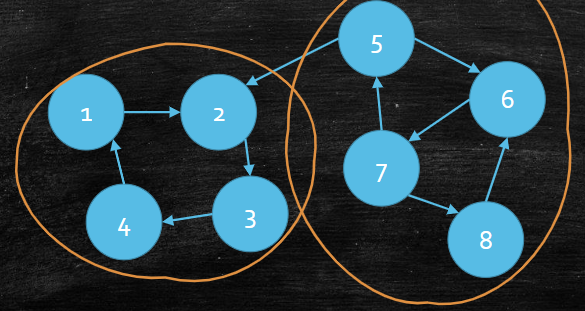
\includegraphics[width=0.8\linewidth]{Notes/fig/SCC.png}
        \caption{SCC}
        \label{fig:SCC}
    \end{minipage}
    \begin{minipage}{0.5\linewidth}
        \centering
        \label{fig:dijk}
        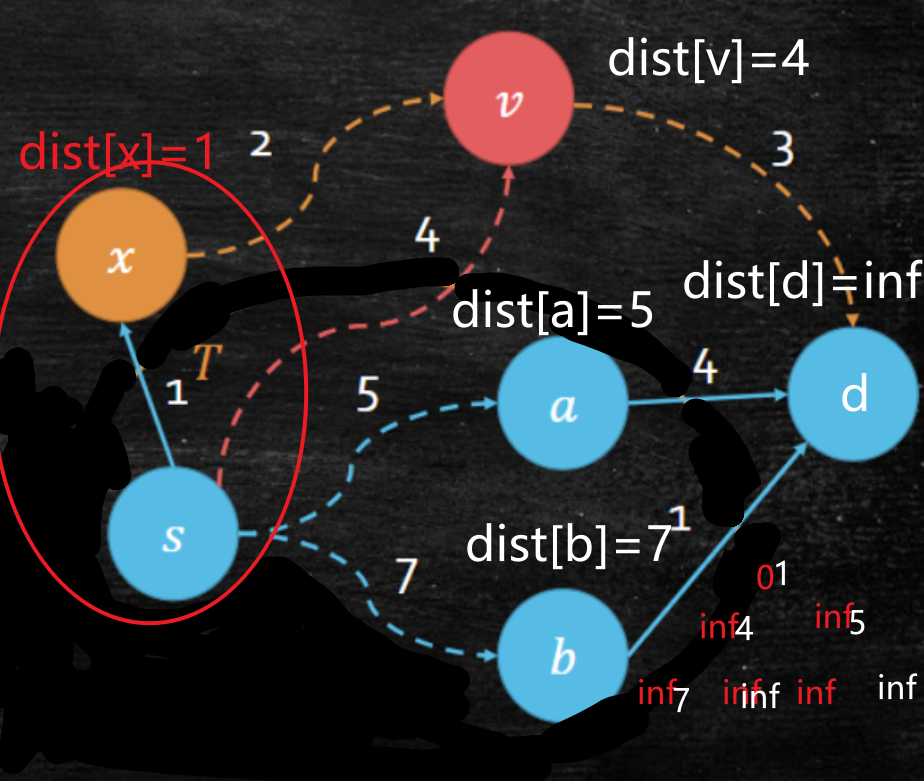
\includegraphics[width=0.5\linewidth]{Notes/fig/dijk.png}
        \caption{Correctness of Dijkstra's algorithm}
    \end{minipage}
\end{figure}




\subsubsection{Dijkstra: SP. with positive weight}
\begin{remark} \textbf{difference between quantity and numerical value}\\
    Pay attention to the length of a numerical value. i.e., input length is $n$, the actual number complexity.
    Storing $n$ quantities takes n storage space, but storing a n-length numerical value takes $\log n$ bits. Therefore, an increase in bits takes exponencial time complexity.
    $O(|V|+|E|)$ , $|`|$ is a quantity
    $O(w_max)$ is a numerical value.
\end{remark}

\begin{itemize}
    \item Works by keep dragging the closest vertex to the current SPT and updating the minimum path length. 
    \item Dijkstra algorithm is based on the assumption that evrey step out of SPT(shortest path tree) at least increases the path length, so it only solves graphs without negative cycles.
    \item A trick is to use heap (binary-heap, d-heap, Fibonachi-heap) to store the shortest distance from other vertice to $s$, so that we can quickly obtain the closest node from SPT, without the need to traverse all outer edges again. 
    Creating the heap takes $O(|V|\log |V|)$, picking the top vertex takes $O(\log |V|)$, and updating all the nodes takes $O((|V|+|E|)\log |V|)$.
    i.e, for figure \ref{fig:dijk},  consider the first step. We update {x,a,b,v} and the closest vertex x natually pops to the top.
\end{itemize}
\textbf{Correctness of algorithm:}
If there exists $x \notin SPT, v \in SPT$, s.t. $dist(s\rightarrow x \rightarrow v)<dist(v)$, $dist(x)<dist(v)$, $x$ should be in $SPT$,contradiction! 
\begin{algorithm}
\caption{Di(j)kstra}
\KwIn{G=(V,E),s}
\KwOut{dist(u) is the shortest distance from s to u}
\# initialize
\ForEach{$u \in V$}{
    dist(u)=$\inf$\\
    pre(u)=Nan
}
dist(s)=0\\
H=makequeue(V)\\
\While{H is not empty}{
    u=H.top();H.pop()\\
    \ForEach{$(u,v) \in E$}{
        \If{$dist(v)>dist(u)+l(u,v)$}{
            $dist(v)=dist(u)+l(u,v)$ \# update the shortest dist \\
            pre(v)=u\# record previous node\\
        }
    }
}

\end{algorithm}

\subsubsection{Bellman-Ford: shortest path with negative weight}
Dijkstra's algorithm works because the dist value it maintains is either overestimates or exactly correct.
The key idea of Bellman-Ford is that it updates all the edges (kind of 'edgewise' operation) each time (different from Dijkstra's algorithm who updates nodes one step connected to SPT), which takes $O(|V||E|)$.

\begin{algorithm}
    \KwIn{G=(V,E),s}
    dist[s]=0, dist[x]=$\inf$ for vertex other than s\\
    pre(v)=Nan\\
    \While{some dist[x] updates}{ \# update at most |V| rounds.
        \ForEach{$(u,v) \in E$}{
            \If{dist[v]>dist[u]+w(u,v)}{
                dist[v]=dist[u]+w(u,v)\\
                pre(v)=u\\
            }
        }
    }
\end{algorithm}
\textbf{Correctness of algorithm:}
\begin{enumerate}
    \item After k rounds, dist(v) is the shortest path of all k-edge-paths.($dist[u_k]\leq d(u_1,u_2,\ldots,u_k)$)
    For base step, dist[s] is the shortest dist of all 0-edge-paths.\\
    For induction step, suppose it is true for $k-1$ rounds, $dist[u_{k-1}] \leq d(u_1,\ldots,u_{k-1})$. By Bellman-ford update condition, $dist[u_{k}]\leq d(u_1,\ldots,u_{k-1})+w(u_{k-1},v)$, the righthand side means all the other k-edge-paths.
    \item For graphs without negative cycle, all the shortest paths will have at most $|V|-1$ edges.
    If there are more than $|V|$ paths, a vertex must be visited twice, but by erasing the whole cycle results in a shorter path, contradiction!
    \item Negative cycle exists iff some dist is updated in the last($|V|^{th}$) round.
    \item If no vertice updates in $V^{th}$ round, then no vertice will be updated then. But if a single vertice is not updated.
    \item If a vertex is upgraded after $V$ rounds, then its path must include a negative cycle.
    A negative cycle can be found by tracing the recorded shortest path until two repeated nodes occurs. Tricks include running till the $2|V|^{th}$ round and see the vertice upgraded in $|V|^{th}$ and $2|V|^th$.
\end{enumerate}
